%!TEX program = pdflatex
\documentclass[11pt,a4paper]{article}

% =============================================================================
% PACKAGES
% =============================================================================

% Page geometry and layout
\usepackage[margin=2.5cm]{geometry}
\usepackage{parskip}
\usepackage{multicol}
\usepackage{fancyhdr}
\usepackage{lastpage}

% Fonts - use standard LaTeX fonts
\usepackage[T1]{fontenc}
\usepackage{lmodern}
\usepackage{inconsolata}

% Math
\usepackage{amsmath,amssymb,amsthm}
\usepackage{mathtools}
\usepackage{bm}

% Colors
\usepackage[dvipsnames,svgnames,x11names]{xcolor}

% Define custom colors
\definecolor{jpegblue}{RGB}{0, 102, 204}
\definecolor{jpegred}{RGB}{204, 51, 51}
\definecolor{jpegorange}{RGB}{230, 126, 34}
\definecolor{jpeggreen}{RGB}{39, 174, 96}
\definecolor{jpegpurple}{RGB}{142, 68, 173}
\definecolor{codebg}{RGB}{248, 248, 248}
\definecolor{codecomment}{RGB}{106, 153, 85}
\definecolor{codestring}{RGB}{163, 21, 21}
\definecolor{codekeyword}{RGB}{0, 0, 255}
\definecolor{darkbg}{RGB}{40, 44, 52}
\definecolor{lightborder}{RGB}{200, 200, 200}

% Graphics and diagrams
\usepackage{tikz}
\usetikzlibrary{
    shapes.geometric,
    arrows.meta,
    positioning,
    calc,
    decorations.pathreplacing,
    backgrounds,
    fit,
    matrix,
    patterns,
    shadows
}
\usepackage{pgfplots}
\pgfplotsset{compat=1.18}

% Boxes and frames
\usepackage[most]{tcolorbox}
\tcbuselibrary{listings,skins,breakable}

% Code listings
\usepackage{listings}
\lstset{
    basicstyle=\ttfamily\small,
    backgroundcolor=\color{codebg},
    commentstyle=\color{codecomment},
    keywordstyle=\color{codekeyword}\bfseries,
    stringstyle=\color{codestring},
    numbers=left,
    numberstyle=\tiny\color{gray},
    numbersep=8pt,
    breaklines=true,
    frame=single,
    framerule=0.5pt,
    rulecolor=\color{lightborder},
    showstringspaces=false,
    tabsize=4,
    xleftmargin=15pt,
    framexleftmargin=15pt
}

\lstdefinestyle{python}{
    language=Python,
    morekeywords={self,True,False,None,as,with,yield,async,await}
}

% Tables
\usepackage{booktabs}
\usepackage{array}
\usepackage{colortbl}
\usepackage{multirow}
\usepackage{tabularx}

% Floats
\usepackage{float}
\usepackage{caption}
\usepackage{subcaption}
\captionsetup{font=small,labelfont=bf}

% Links
\usepackage{hyperref}
\hypersetup{
    colorlinks=true,
    linkcolor=jpegblue,
    urlcolor=jpegpurple,
    citecolor=jpeggreen,
    pdfauthor={Sami Hindi},
    pdftitle={Comprehensive JPEG Encoder Implementation},
    pdfsubject={Image Compression}
}

% Misc
\usepackage{enumitem}

% =============================================================================
% CUSTOM TCOLORBOXES
% =============================================================================

% Main section box
\newtcolorbox{sectionbox}[2][]{
    enhanced,
    colback=white,
    colframe=jpegblue,
    fonttitle=\bfseries\large,
    title=#2,
    attach boxed title to top left={yshift=-2mm,xshift=5mm},
    boxed title style={colback=jpegblue,colframe=jpegblue,sharp corners},
    sharp corners,
    boxrule=1pt,
    top=4mm,
    #1
}

% Definition box
\newtcolorbox{definitionbox}[1][]{
    enhanced,
    colback=blue!5,
    colframe=jpegblue!70,
    fonttitle=\bfseries,
    title=Definition,
    left=3mm,
    right=3mm,
    boxrule=0.5pt,
    leftrule=4pt,
    arc=0pt,
    #1
}

% Formula box
\newtcolorbox{formulabox}[1][]{
    enhanced,
    colback=orange!5,
    colframe=jpegorange!70,
    boxrule=0.5pt,
    leftrule=4pt,
    arc=0pt,
    left=3mm,
    right=3mm,
    #1
}

% Warning box
\newtcolorbox{warningbox}[1][]{
    enhanced,
    colback=red!5,
    colframe=jpegred!70,
    fonttitle=\bfseries,
    title={Warning},
    boxrule=0.5pt,
    leftrule=4pt,
    arc=0pt,
    #1
}

% Code box
\newtcblisting{pythoncode}[1][]{
    enhanced,
    listing engine=listings,
    listing only,
    listing options={style=python,#1},
    colback=codebg,
    colframe=lightborder,
    boxrule=0.5pt,
    arc=2pt,
    left=2mm,
    right=2mm,
    top=1mm,
    bottom=1mm
}

% Algorithm box
\newtcolorbox{algorithmbox}[2][]{
    enhanced,
    colback=purple!3,
    colframe=jpegpurple!70,
    fonttitle=\bfseries,
    title={Algorithm: #2},
    boxrule=0.5pt,
    arc=2pt,
    #1
}

% =============================================================================
% HEADER/FOOTER
% =============================================================================

\pagestyle{fancy}
\fancyhf{}
\fancyhead[L]{\small\textcolor{gray}{JPEG Encoder Implementation}}
\fancyhead[R]{\small\textcolor{gray}{\nouppercase{\leftmark}}}
\fancyfoot[C]{\small\textcolor{gray}{Page \thepage\ of \pageref{LastPage}}}
\renewcommand{\headrulewidth}{0.4pt}
\renewcommand{\footrulewidth}{0.4pt}

% =============================================================================
% DOCUMENT
% =============================================================================

\begin{document}

% Custom title page
\begin{titlepage}

\begin{tikzpicture}[remember picture,overlay]
    % Background gradient
    \fill[left color=jpegblue!80,right color=jpegpurple!60]
        (current page.south west) rectangle (current page.north east);

    % Decorative circles
    \foreach \i in {1,...,15} {
        \pgfmathsetmacro{\xpos}{rand*10-5}
        \pgfmathsetmacro{\ypos}{rand*14-7}
        \pgfmathsetmacro{\radius}{0.5+rand*2}
        \fill[white,opacity=0.05] (\xpos,\ypos) circle (\radius);
    }

    % Title box
    \node[
        fill=white,
        rounded corners=5pt,
        inner sep=20pt,
        drop shadow={shadow xshift=2pt,shadow yshift=-2pt,opacity=0.3}
    ] at (current page.center) {
        \begin{minipage}{0.8\textwidth}
            \centering
            {\fontsize{36}{44}\selectfont\bfseries\textcolor{jpegblue}{JPEG Encoder}}\\[8pt]
            {\fontsize{18}{22}\selectfont\textcolor{gray}{Comprehensive Implementation Guide}}\\[20pt]
            \rule{0.6\textwidth}{1pt}\\[20pt]
            {\large From Pixels to Compressed Bytes}\\[10pt]
            {\small A Deep Dive into DCT, Quantization, and Huffman Coding}\\[30pt]
            {\normalsize\textcolor{gray}{Python Implementation with Mathematical Foundation}}\\[10pt]
            {\small\today}\\[5pt]
            {\normalsize\textcolor{gray}{Sami Hindi}}
        \end{minipage}
    };

    % Bottom decoration
    \node[white,opacity=0.8] at ([yshift=2cm]current page.south) {
        \Large\texttt{jpeg.py}
    };
\end{tikzpicture}
\end{titlepage}

% =============================================================================
% TABLE OF CONTENTS
% =============================================================================

\tableofcontents
\newpage

% =============================================================================
% INTRODUCTION
% =============================================================================

\section{Introduction}

\begin{sectionbox}{What is JPEG?}
\textbf{JPEG} (Joint Photographic Experts Group) is a widely-used lossy compression
standard for digital images. It achieves significant file size reduction by exploiting
characteristics of human vision---we are more sensitive to brightness changes than
color changes, and less sensitive to high-frequency details.

\vspace{2mm}
The JPEG algorithm consists of several key stages:
\begin{enumerate}[leftmargin=2cm]
    \item \textcolor{jpegblue}{\textbf{Color Space Conversion}} --- RGB to YCbCr
    \item \textcolor{jpegorange}{\textbf{Chroma Subsampling}} --- Reduce color resolution
    \item \textcolor{jpeggreen}{\textbf{Block Splitting}} --- Divide into 8$\times$8 blocks
    \item \textcolor{jpegpurple}{\textbf{DCT Transform}} --- Convert to frequency domain
    \item \textcolor{jpegred}{\textbf{Quantization}} --- Reduce precision (lossy step)
    \item \textcolor{jpegblue}{\textbf{Entropy Coding}} --- Huffman compression
\end{enumerate}
\end{sectionbox}

\subsection{Encoding Pipeline Overview}

\begin{figure}[H]
\centering
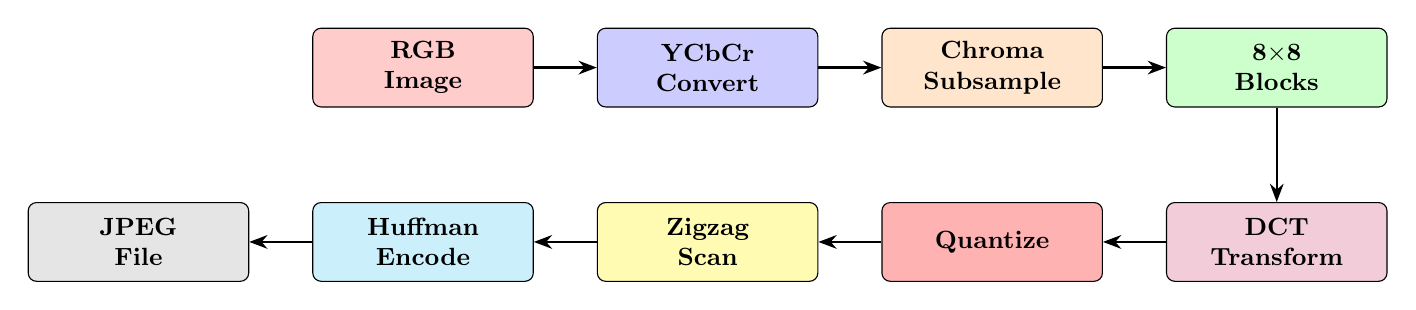
\begin{tikzpicture}[
    node distance=0.8cm,
    block/.style={
        rectangle,
        draw,
        rounded corners=3pt,
        minimum width=2.8cm,
        minimum height=1cm,
        align=center,
        font=\small\bfseries
    },
    arrow/.style={->,>=Stealth,thick}
]
    % Nodes
    \node[block,fill=red!20] (input) {RGB\\Image};
    \node[block,fill=blue!20,right=of input] (ycbcr) {YCbCr\\Convert};
    \node[block,fill=orange!20,right=of ycbcr] (subsample) {Chroma\\Subsample};
    \node[block,fill=green!20,right=of subsample] (blocks) {8$\times$8\\Blocks};

    \node[block,fill=purple!20,below=1.2cm of blocks] (dct) {DCT\\Transform};
    \node[block,fill=red!30,left=of dct] (quant) {Quantize};
    \node[block,fill=yellow!30,left=of quant] (zigzag) {Zigzag\\Scan};
    \node[block,fill=cyan!20,left=of zigzag] (huffman) {Huffman\\Encode};
    \node[block,fill=gray!20,left=of huffman] (output) {JPEG\\File};

    % Arrows
    \draw[arrow] (input) -- (ycbcr);
    \draw[arrow] (ycbcr) -- (subsample);
    \draw[arrow] (subsample) -- (blocks);
    \draw[arrow] (blocks) -- (dct);
    \draw[arrow] (dct) -- (quant);
    \draw[arrow] (quant) -- (zigzag);
    \draw[arrow] (zigzag) -- (huffman);
    \draw[arrow] (huffman) -- (output);
\end{tikzpicture}
\caption{JPEG encoding pipeline showing the transformation from RGB input to compressed output.}
\label{fig:pipeline}
\end{figure}

% =============================================================================
% COLOR SPACE CONVERSION
% =============================================================================

\newpage
\section{Color Space Conversion}
\label{sec:colorspace}

\begin{sectionbox}{RGB to YCbCr Transformation}
Human vision is more sensitive to luminance (brightness) than chrominance (color).
JPEG exploits this by separating the image into:

\begin{itemize}
    \item \textbf{Y} --- Luminance (brightness)
    \item \textbf{Cb} --- Blue-difference chroma component
    \item \textbf{Cr} --- Red-difference chroma component
\end{itemize}
\end{sectionbox}

\subsection{Mathematical Formulation}

The ITU-R BT.601 standard defines the conversion:

\begin{formulabox}
\begin{equation}
\begin{bmatrix} Y \\ C_b \\ C_r \end{bmatrix} =
\begin{bmatrix}
0.299 & 0.587 & 0.114 \\
-0.169 & -0.331 & 0.5 \\
0.5 & -0.419 & -0.081
\end{bmatrix}
\begin{bmatrix} R \\ G \\ B \end{bmatrix} +
\begin{bmatrix} 0 \\ 128 \\ 128 \end{bmatrix}
\label{eq:rgb2ycbcr}
\end{equation}
\end{formulabox}

\begin{definitionbox}
The coefficients in the Y row (0.299, 0.587, 0.114) reflect human perception---we are
most sensitive to green, then red, then blue.
\end{definitionbox}

\subsection{Implementation}

\begin{pythoncode}
def rgb_to_ycbcr(rgb: np.ndarray) -> np.ndarray:
    """Convert RGB to YCbCr color space."""
    transform = np.array([
        [0.299, 0.587, 0.114],
        [-0.169, -0.331, 0.5],
        [0.5, -0.419, -0.081]
    ])
    ycbcr = np.zeros_like(rgb, dtype=np.float64)
    # Apply matrix transformation
    for i in range(3):
        ycbcr[:,:,i] = sum(transform[i,j] * rgb[:,:,j]
                          for j in range(3))
    ycbcr[:,:,1:] += 128  # Offset chroma
    return np.clip(ycbcr, 0, 255)
\end{pythoncode}

% =============================================================================
% CHROMA SUBSAMPLING
% =============================================================================

\newpage
\section{Chroma Subsampling}
\label{sec:subsampling}

\begin{sectionbox}{Reducing Color Resolution}
Since human vision has lower spatial resolution for color than brightness, we can
reduce the resolution of the Cb and Cr channels with minimal perceptual impact.
\end{sectionbox}

\subsection{Subsampling Modes}

\begin{figure}[H]
\centering
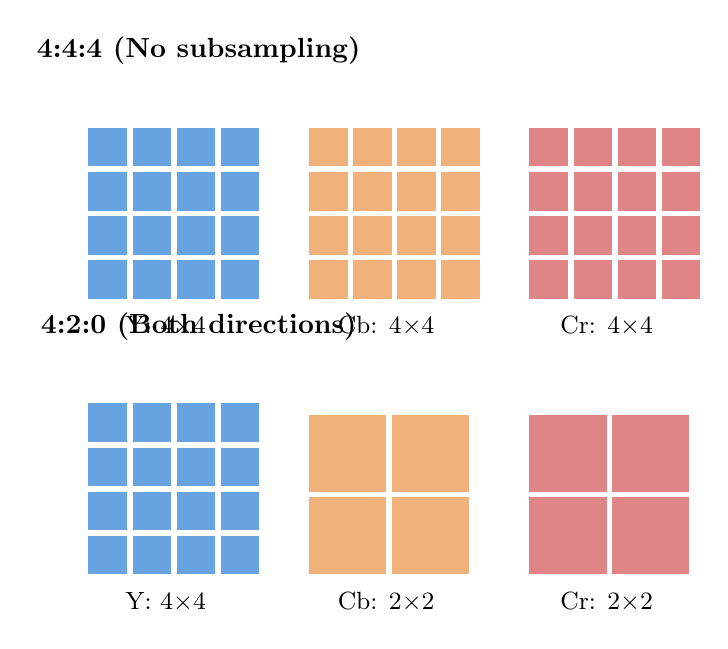
\begin{tikzpicture}[scale=0.7]
    % 4:4:4
    \begin{scope}
        \node[font=\bfseries] at (2,4.5) {4:4:4 (No subsampling)};
        \foreach \x in {0,...,3} {
            \foreach \y in {0,...,3} {
                \fill[jpegblue!60] (\x*0.8,\y*0.8) rectangle (\x*0.8+0.7,\y*0.8+0.7);
            }
        }
        \node at (1.4,-0.5) {\small Y: 4$\times$4};

        \begin{scope}[xshift=4cm]
        \foreach \x in {0,...,3} {
            \foreach \y in {0,...,3} {
                \fill[jpegorange!60] (\x*0.8,\y*0.8) rectangle (\x*0.8+0.7,\y*0.8+0.7);
            }
        }
        \node at (1.4,-0.5) {\small Cb: 4$\times$4};
        \end{scope}

        \begin{scope}[xshift=8cm]
        \foreach \x in {0,...,3} {
            \foreach \y in {0,...,3} {
                \fill[jpegred!60] (\x*0.8,\y*0.8) rectangle (\x*0.8+0.7,\y*0.8+0.7);
            }
        }
        \node at (1.4,-0.5) {\small Cr: 4$\times$4};
        \end{scope}
    \end{scope}

    % 4:2:0
    \begin{scope}[yshift=-5cm]
        \node[font=\bfseries] at (2,4.5) {4:2:0 (Both directions)};
        \foreach \x in {0,...,3} {
            \foreach \y in {0,...,3} {
                \fill[jpegblue!60] (\x*0.8,\y*0.8) rectangle (\x*0.8+0.7,\y*0.8+0.7);
            }
        }
        \node at (1.4,-0.5) {\small Y: 4$\times$4};

        \begin{scope}[xshift=4cm]
        \foreach \x in {0,...,1} {
            \foreach \y in {0,...,1} {
                \fill[jpegorange!60] (\x*1.5,\y*1.5) rectangle (\x*1.5+1.4,\y*1.5+1.4);
            }
        }
        \node at (1.4,-0.5) {\small Cb: 2$\times$2};
        \end{scope}

        \begin{scope}[xshift=8cm]
        \foreach \x in {0,...,1} {
            \foreach \y in {0,...,1} {
                \fill[jpegred!60] (\x*1.5,\y*1.5) rectangle (\x*1.5+1.4,\y*1.5+1.4);
            }
        }
        \node at (1.4,-0.5) {\small Cr: 2$\times$2};
        \end{scope}
    \end{scope}
\end{tikzpicture}
\caption{Comparison of chroma subsampling modes. 4:2:0 reduces chroma data to 25\% of original.}
\label{fig:subsampling}
\end{figure}

\begin{table}[H]
\centering
\caption{Subsampling Mode Comparison}
\begin{tabular}{@{}lccc@{}}
\toprule
\textbf{Mode} & \textbf{H Ratio} & \textbf{V Ratio} & \textbf{Data Reduction} \\
\midrule
4:4:4 & 1:1 & 1:1 & None \\
4:2:2 & 2:1 & 1:1 & 33\% \\
\rowcolor{jpegblue!10}
4:2:0 & 2:1 & 2:1 & 50\% \\
\bottomrule
\end{tabular}
\end{table}

% =============================================================================
% DISCRETE COSINE TRANSFORM
% =============================================================================

\newpage
\section{Discrete Cosine Transform (DCT)}
\label{sec:dct}

\begin{sectionbox}{Frequency Domain Transformation}
The DCT converts spatial pixel values into frequency coefficients. Low frequencies
(upper-left of the block) represent smooth gradients, while high frequencies
(lower-right) represent sharp edges and details.
\end{sectionbox}

\subsection{2D-DCT Formula}

The two-dimensional DCT-II for an $N \times N$ block is defined as:

\begin{formulabox}
\begin{equation}
F(u,v) = \frac{1}{4} C(u) C(v) \sum_{x=0}^{N-1} \sum_{y=0}^{N-1} f(x,y)
\cos\left[\frac{(2x+1)u\pi}{2N}\right]
\cos\left[\frac{(2y+1)v\pi}{2N}\right]
\label{eq:dct}
\end{equation}
\end{formulabox}

where:
\begin{align}
C(k) &= \begin{cases} \frac{1}{\sqrt{2}} & \text{if } k = 0 \\ 1 & \text{otherwise} \end{cases}
\end{align}

\begin{definitionbox}
The coefficient $F(0,0)$ is called the \textbf{DC coefficient} and represents the
average value of the block. All other coefficients are \textbf{AC coefficients}.
\end{definitionbox}

\subsection{DCT Basis Functions}

\begin{figure}[H]
\centering
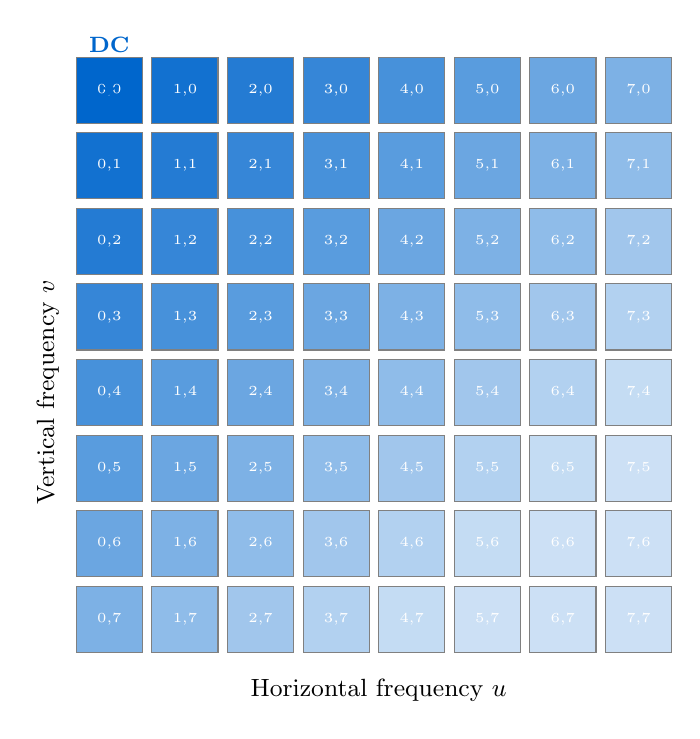
\begin{tikzpicture}[scale=0.6]
    % Draw 8x8 grid of basis function representations
    \foreach \u in {0,...,7} {
        \foreach \v in {0,...,7} {
            \pgfmathsetmacro{\freq}{\u+\v}
            \pgfmathsetmacro{\fillop}{max(20,100-\freq*7)}
            \fill[jpegblue!\fillop] (\u*1.6,7*1.6-\v*1.6) rectangle (\u*1.6+1.4,7*1.6-\v*1.6+1.4);
            \draw[gray,thin] (\u*1.6,7*1.6-\v*1.6) rectangle (\u*1.6+1.4,7*1.6-\v*1.6+1.4);
            \node[font=\tiny,white] at (\u*1.6+0.7,7*1.6-\v*1.6+0.7) {\u,\v};
        }
    }
    \node[rotate=90] at (-0.6,5.5) {\small Vertical frequency $v$};
    \node at (6.4,-0.8) {\small Horizontal frequency $u$};

    % DC label
    \node[above,font=\footnotesize\bfseries,jpegblue] at (0.7,12.5) {DC};
    \draw[->,thick,jpegblue] (0.7,12.3) -- (0.7,11.8);
\end{tikzpicture}
\caption{The 64 DCT basis function positions. $(u,v)$ indicates frequency indices.
Upper-left (0,0) is DC; frequency increases toward lower-right.}
\label{fig:dct_basis}
\end{figure}

\subsection{Matrix Implementation}

For efficiency, the 2D-DCT is computed using matrix multiplication:

\begin{formulabox}
\begin{equation}
\mathbf{F} = \mathbf{D} \cdot \mathbf{f} \cdot \mathbf{D}^T
\end{equation}
\end{formulabox}

where $\mathbf{D}$ is the DCT transformation matrix:

\begin{equation}
D_{ij} = \begin{cases}
\frac{1}{\sqrt{N}} & \text{if } i = 0 \\[4pt]
\sqrt{\frac{2}{N}} \cos\left[\frac{(2j+1)i\pi}{2N}\right] & \text{otherwise}
\end{cases}
\end{equation}

\subsection{Implementation}

\begin{pythoncode}
def create_dct_matrix(n: int = 8) -> np.ndarray:
    """Create the DCT-II transformation matrix."""
    dct_matrix = np.zeros((n, n), dtype=np.float64)
    for i in range(n):
        for j in range(n):
            if i == 0:
                dct_matrix[i, j] = 1 / np.sqrt(n)
            else:
                dct_matrix[i, j] = np.sqrt(2/n) * \
                    np.cos((2*j + 1) * i * np.pi / (2*n))
    return dct_matrix

DCT_MATRIX = create_dct_matrix(8)

def dct_2d(block: np.ndarray) -> np.ndarray:
    """Apply 2D DCT: F = D * f * D^T"""
    return DCT_MATRIX @ block @ DCT_MATRIX.T
\end{pythoncode}

% =============================================================================
% QUANTIZATION
% =============================================================================

\newpage
\section{Quantization}
\label{sec:quantization}

\begin{sectionbox}{The Lossy Step}
Quantization is where JPEG achieves most of its compression---and where information
is permanently lost. Each DCT coefficient is divided by a quantization value and
rounded to an integer.
\end{sectionbox}

\subsection{Quantization Formula}

\begin{formulabox}
\begin{equation}
F_Q(u,v) = \text{round}\left(\frac{F(u,v)}{Q(u,v)}\right)
\label{eq:quant}
\end{equation}
\end{formulabox}

\subsection{Standard Quantization Tables}

\begin{figure}[H]
\centering
\begin{minipage}{0.48\textwidth}
\centering
\textbf{Luminance (Y)}
\vspace{2mm}

\begin{tikzpicture}[scale=0.48]
\def\lumtable{
    {16,11,10,16,24,40,51,61},
    {12,12,14,19,26,58,60,55},
    {14,13,16,24,40,57,69,56},
    {14,17,22,29,51,87,80,62},
    {18,22,37,56,68,109,103,77},
    {24,35,55,64,81,104,113,92},
    {49,64,78,87,103,121,120,101},
    {72,92,95,98,112,100,103,99}
}

\foreach \row [count=\j from 0] in \lumtable {
    \foreach \val [count=\i from 0] in \row {
        \pgfmathsetmacro{\intensity}{max(20,100-\val*0.7)}
        \fill[jpegblue!\intensity] (\i,7-\j) rectangle (\i+0.95,7-\j+0.95);
        \node[font=\tiny,white] at (\i+0.475,7-\j+0.475) {\val};
    }
}
\draw[black,thick] (0,0) rectangle (8,8);
\end{tikzpicture}
\end{minipage}
\hfill
\begin{minipage}{0.48\textwidth}
\centering
\textbf{Chrominance (Cb, Cr)}
\vspace{2mm}

\begin{tikzpicture}[scale=0.48]
\def\chrtable{
    {17,18,24,47,99,99,99,99},
    {18,21,26,66,99,99,99,99},
    {24,26,56,99,99,99,99,99},
    {47,66,99,99,99,99,99,99},
    {99,99,99,99,99,99,99,99},
    {99,99,99,99,99,99,99,99},
    {99,99,99,99,99,99,99,99},
    {99,99,99,99,99,99,99,99}
}

\foreach \row [count=\j from 0] in \chrtable {
    \foreach \val [count=\i from 0] in \row {
        \pgfmathsetmacro{\intensity}{max(20,100-\val*0.7)}
        \fill[jpegorange!\intensity] (\i,7-\j) rectangle (\i+0.95,7-\j+0.95);
        \node[font=\tiny,white] at (\i+0.475,7-\j+0.475) {\val};
    }
}
\draw[black,thick] (0,0) rectangle (8,8);
\end{tikzpicture}
\end{minipage}
\caption{Standard JPEG quantization tables (ITU-T T.81). Higher values = more compression.}
\label{fig:quant_tables}
\end{figure}

\subsection{Quality Scaling}

The quality parameter (1--100) scales the quantization table:

\begin{formulabox}
\begin{equation}
Q_{\text{scaled}}(u,v) = \text{clip}\left(\left\lfloor\frac{Q(u,v) \cdot S + 50}{100}\right\rfloor, 1, 255\right)
\end{equation}
where $S = \begin{cases} \frac{5000}{q} & \text{if } q < 50 \\ 200 - 2q & \text{if } q \geq 50 \end{cases}$
\end{formulabox}

% =============================================================================
% ZIGZAG AND RLE
% =============================================================================

\newpage
\section{Zigzag Scanning \& Run-Length Encoding}
\label{sec:zigzag}

\begin{sectionbox}{Preparing for Entropy Coding}
After quantization, many high-frequency coefficients become zero. The zigzag scan
orders coefficients from low to high frequency, grouping zeros together for efficient
run-length encoding.
\end{sectionbox}

\subsection{Zigzag Pattern}

\begin{figure}[H]
\centering
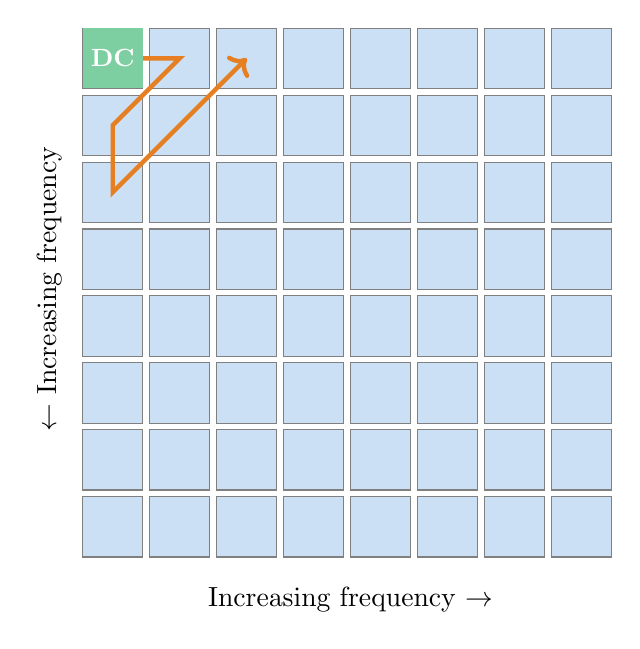
\begin{tikzpicture}[scale=0.85]
    % Grid with numbers
    \def\zigzag{
        0,  1,  5,  6, 14, 15, 27, 28,
        2,  4,  7, 13, 16, 26, 29, 42,
        3,  8, 12, 17, 25, 30, 41, 43,
        9, 11, 18, 24, 31, 40, 44, 53,
       10, 19, 23, 32, 39, 45, 52, 54,
       20, 22, 33, 38, 46, 51, 55, 60,
       21, 34, 37, 47, 50, 56, 59, 61,
       35, 36, 48, 49, 57, 58, 62, 63
    }

    \foreach \x in {0,...,7} {
        \foreach \y in {0,...,7} {
            \pgfmathsetmacro{\idx}{int(\y*8+\x)}
            \fill[jpegblue!20] (\x,7-\y) rectangle (\x+0.9,7-\y+0.9);
            \draw[gray] (\x,7-\y) rectangle (\x+0.9,7-\y+0.9);
        }
    }

    % Draw zigzag path (simplified)
    \draw[jpegorange,ultra thick,->]
        (0.45,7.45) -- (1.45,7.45) -- (0.45,6.45) -- (0.45,5.45) --
        (1.45,6.45) -- (2.45,7.45);

    % DC label
    \fill[jpeggreen!60] (0,7) rectangle (0.9,7.9);
    \node[font=\small\bfseries,white] at (0.45,7.45) {DC};

    % Labels
    \node[below] at (4,-0.3) {Increasing frequency $\rightarrow$};
    \node[rotate=90] at (-0.5,4) {$\leftarrow$ Increasing frequency};
\end{tikzpicture}
\caption{Zigzag scan begins at DC (green) and proceeds toward high frequencies.}
\label{fig:zigzag}
\end{figure}

\subsection{Run-Length Encoding}

AC coefficients are encoded as (run, value) pairs:

\begin{algorithmbox}{RLE for AC Coefficients}
\begin{enumerate}
    \item Start after DC coefficient (position 1)
    \item Count consecutive zeros (run length)
    \item Encode: (run\_length, size, value)
    \item If run $>$ 15: emit ZRL symbol (15, 0) and continue
    \item End with EOB symbol (0, 0) if trailing zeros
\end{enumerate}
\end{algorithmbox}

\begin{definitionbox}
\textbf{Example:} Coefficients \texttt{[DC, 5, 0, 0, -3, 0, 0, 0, 0, 1, 0...0]}

Encoded as: \texttt{(0,3,5), (2,2,-3), (4,1,1), EOB}
\end{definitionbox}

% =============================================================================
% HUFFMAN ENCODING
% =============================================================================

\newpage
\section{Huffman Encoding}
\label{sec:huffman}

\begin{sectionbox}{Entropy Coding}
Huffman coding assigns shorter bit sequences to more frequent symbols. JPEG uses
separate tables for DC and AC coefficients, and for luminance and chrominance.
\end{sectionbox}

\subsection{DC Coefficient Encoding}

DC coefficients are encoded \textbf{differentially}---each DC value is the difference
from the previous block's DC:

\begin{formulabox}
\begin{equation}
\text{DIFF} = \text{DC}_n - \text{DC}_{n-1}
\end{equation}
\end{formulabox}

The difference is encoded as:
\begin{enumerate}
    \item Huffman code for the \textbf{size} (number of bits needed)
    \item The actual \textbf{value} in that many bits
\end{enumerate}

\subsection{Standard DC Luminance Huffman Table}

\begin{table}[H]
\centering
\caption{DC Luminance Huffman Codes (Partial)}
\begin{tabular}{@{}cccl@{}}
\toprule
\textbf{Size} & \textbf{Code Length} & \textbf{Code (binary)} & \textbf{Value Range} \\
\midrule
0 & 2 & \texttt{00} & 0 \\
1 & 3 & \texttt{010} & $-1, 1$ \\
2 & 3 & \texttt{011} & $-3..-2, 2..3$ \\
3 & 3 & \texttt{100} & $-7..-4, 4..7$ \\
4 & 3 & \texttt{101} & $-15..-8, 8..15$ \\
5 & 3 & \texttt{110} & $-31..-16, 16..31$ \\
6 & 4 & \texttt{1110} & $-63..-32, 32..63$ \\
\bottomrule
\end{tabular}
\end{table}

\subsection{Bit Writing with Byte Stuffing}

\begin{warningbox}
JPEG requires \textbf{byte stuffing}: whenever \texttt{0xFF} appears in the entropy-coded
data, it must be followed by \texttt{0x00} to distinguish it from markers.
\end{warningbox}

\begin{pythoncode}
class BitWriter:
    def write_bits(self, value: int, num_bits: int):
        self.bit_buffer = (self.bit_buffer << num_bits) | value
        self.bit_count += num_bits

        while self.bit_count >= 8:
            self.bit_count -= 8
            byte = (self.bit_buffer >> self.bit_count) & 0xFF
            self.buffer.append(byte)
            # Byte stuffing: 0xFF -> 0xFF 0x00
            if byte == 0xFF:
                self.buffer.append(0x00)
\end{pythoncode}

% =============================================================================
% JPEG FILE STRUCTURE
% =============================================================================

\newpage
\section{JPEG File Structure}
\label{sec:filestructure}

\begin{sectionbox}{JFIF Format}
A JPEG file consists of segments, each beginning with a two-byte marker. The JFIF
(JPEG File Interchange Format) is the most common container format.
\end{sectionbox}

\subsection{Marker Overview}

\begin{figure}[H]
\centering
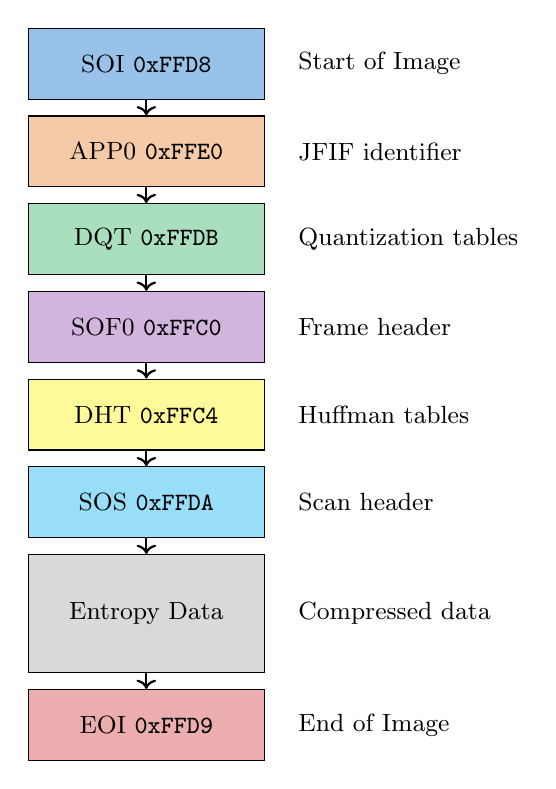
\begin{tikzpicture}[
    block/.style={
        rectangle, draw, minimum width=3cm, minimum height=0.9cm,
        align=center, font=\small
    }
]
    \node[block,fill=jpegblue!40] (soi) at (0,0) {SOI \texttt{0xFFD8}};
    \node[block,fill=jpegorange!40,below=0.2cm of soi] (app0) {APP0 \texttt{0xFFE0}};
    \node[block,fill=jpeggreen!40,below=0.2cm of app0] (dqt) {DQT \texttt{0xFFDB}};
    \node[block,fill=jpegpurple!40,below=0.2cm of dqt] (sof0) {SOF0 \texttt{0xFFC0}};
    \node[block,fill=yellow!40,below=0.2cm of sof0] (dht) {DHT \texttt{0xFFC4}};
    \node[block,fill=cyan!40,below=0.2cm of dht] (sos) {SOS \texttt{0xFFDA}};
    \node[block,fill=gray!30,below=0.2cm of sos,minimum height=1.5cm] (data) {Entropy Data};
    \node[block,fill=jpegred!40,below=0.2cm of data] (eoi) {EOI \texttt{0xFFD9}};

    % Descriptions
    \node[right=0.3cm of soi,font=\small] {Start of Image};
    \node[right=0.3cm of app0,font=\small] {JFIF identifier};
    \node[right=0.3cm of dqt,font=\small] {Quantization tables};
    \node[right=0.3cm of sof0,font=\small] {Frame header};
    \node[right=0.3cm of dht,font=\small] {Huffman tables};
    \node[right=0.3cm of sos,font=\small] {Scan header};
    \node[right=0.3cm of data,font=\small] {Compressed data};
    \node[right=0.3cm of eoi,font=\small] {End of Image};

    % Arrows
    \foreach \a/\b in {soi/app0,app0/dqt,dqt/sof0,sof0/dht,dht/sos,sos/data,data/eoi} {
        \draw[->,thick] (\a) -- (\b);
    }
\end{tikzpicture}
\caption{JPEG file structure showing marker sequence.}
\label{fig:filestructure}
\end{figure}

\subsection{SOF0 Component Specification}

\begin{table}[H]
\centering
\caption{SOF0 Component Parameters for Different Subsampling Modes}
\begin{tabular}{@{}lcccc@{}}
\toprule
\textbf{Component} & \textbf{ID} & \textbf{4:4:4} & \textbf{4:2:2} & \textbf{4:2:0} \\
\midrule
Y (Luminance)   & 1 & 0x11 & 0x21 & 0x22 \\
Cb (Chroma)     & 2 & 0x11 & 0x11 & 0x11 \\
Cr (Chroma)     & 3 & 0x11 & 0x11 & 0x11 \\
\bottomrule
\end{tabular}
\end{table}

% =============================================================================
% RESULTS
% =============================================================================

\newpage
\section{Implementation Results}
\label{sec:results}

\subsection{Compression Performance}

\begin{figure}[H]
\centering
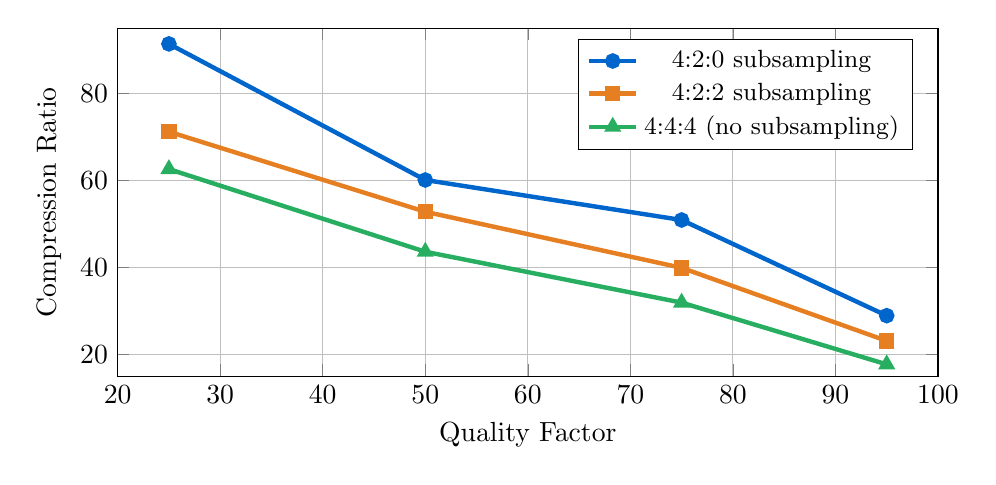
\begin{tikzpicture}
\begin{axis}[
    width=12cm,
    height=6cm,
    xlabel={Quality Factor},
    ylabel={Compression Ratio},
    xmin=20, xmax=100,
    ymin=15, ymax=95,
    grid=major,
    legend pos=north east,
    legend style={font=\small}
]
% 4:2:0
\addplot[jpegblue,ultra thick,mark=*,mark size=2pt] coordinates {
    (25,91.4) (50,60.1) (75,50.9) (95,28.9)
};
% 4:2:2
\addplot[jpegorange,ultra thick,mark=square*,mark size=2pt] coordinates {
    (25,71.2) (50,52.8) (75,39.9) (95,23.1)
};
% 4:4:4
\addplot[jpeggreen,ultra thick,mark=triangle*,mark size=2pt] coordinates {
    (25,62.6) (50,43.6) (75,31.9) (95,17.7)
};
\addlegendentry{4:2:0 subsampling}
\addlegendentry{4:2:2 subsampling}
\addlegendentry{4:4:4 (no subsampling)}
\end{axis}
\end{tikzpicture}
\caption{Compression ratio vs.\ quality factor for different subsampling modes.}
\end{figure}

\subsection{Quality Metrics}

\begin{table}[H]
\centering
\caption{PSNR Results for 256$\times$256 Test Image}
\begin{tabular}{@{}lccc@{}}
\toprule
\textbf{Quality} & \textbf{4:2:0 PSNR} & \textbf{4:2:2 PSNR} & \textbf{4:4:4 PSNR} \\
\midrule
25  & 30.9 dB & 33.4 dB & 39.1 dB \\
50  & 31.9 dB & 34.4 dB & 41.9 dB \\
75  & 32.1 dB & 35.1 dB & 48.4 dB \\
\rowcolor{jpegblue!10}
95  & 32.1 dB & 35.2 dB & 52.0 dB \\
\bottomrule
\end{tabular}
\end{table}

\begin{definitionbox}
\textbf{PSNR} (Peak Signal-to-Noise Ratio) is calculated as:
\begin{equation}
\text{PSNR} = 10 \cdot \log_{10}\left(\frac{255^2}{\text{MSE}}\right) \text{ dB}
\end{equation}
Higher values indicate better quality. Values $>$ 40 dB are considered excellent.
\end{definitionbox}

% =============================================================================
% USAGE
% =============================================================================

\newpage
\section{Usage Guide}

\subsection{Command Line}

\begin{tcolorbox}[colback=darkbg,coltext=white,colframe=darkbg,fontupper=\ttfamily\small]
\# Basic encoding\\
python jpeg.py input.png output.jpg\\
\\
\# High quality, no subsampling\\
python jpeg.py input.png output.jpg -q 95 -s 444\\
\\
\# Generate test image\\
python jpeg.py --test -v
\end{tcolorbox}

\subsection{Python API}

\begin{pythoncode}
from jpeg import encode_image, save_jpeg, SubsamplingMode
import numpy as np

# Load or create image
image = np.random.randint(0, 256, (512, 512, 3), dtype=np.uint8)

# Encode to bytes
jpeg_bytes = encode_image(image, quality=85)

# Save to file
save_jpeg(image, "output.jpg",
          quality=90,
          subsampling=SubsamplingMode.MODE_420)
\end{pythoncode}

% =============================================================================
% REFERENCES
% =============================================================================

\section{References}

\begin{enumerate}[leftmargin=*]
    \item \textbf{ITU-T T.81} --- Digital compression and coding of continuous-tone
          still images: Requirements and guidelines (JPEG standard)
    \item \textbf{ITU-R BT.601} --- Studio encoding parameters of digital television
    \item Wallace, G.K. (1991). \textit{The JPEG Still Picture Compression Standard}.
          Communications of the ACM.
\end{enumerate}

\vfill

\begin{center}
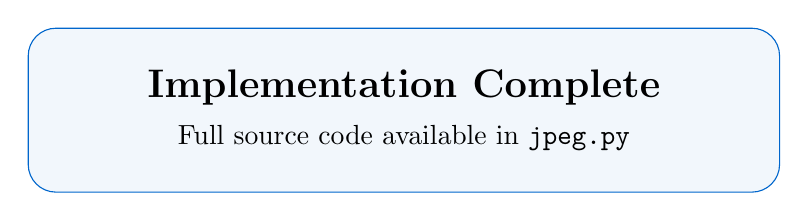
\begin{tikzpicture}
    \node[draw=jpegblue,rounded corners=10pt,inner sep=15pt,fill=jpegblue!5] {
        \begin{minipage}{0.7\textwidth}
            \centering
            \Large\bfseries Implementation Complete\\[5pt]
            \normalsize\normalfont
            Full source code available in \texttt{jpeg.py}
        \end{minipage}
    };
\end{tikzpicture}
\end{center}

\end{document}
